\documentclass[aspectratio=169]{beamer}
\geometry{paperwidth=160mm,paperheight=100mm}
\usepackage{beamerthemesidebar}
\usepackage{hyperref}
\usepackage{color}
\usepackage{multimedia}
\usepackage{colortbl}
\usepackage{amsmath}
\usepackage{empheq}
\usepackage{cancel}
\usepackage{amssymb}
\usepackage{amsfonts}
\usepackage{lipsum}
\usepackage{tcolorbox}
\usepackage{tabularx}
\usepackage{caption}

\setbeamersize{sidebar width right=0pt}
\setbeamertemplate{footline}[frame number]
%
\definecolor{orange}{RGB}{250,167,12}
\definecolor{yellow}{RGB}{246,250,12}
\definecolor{green}{RGB}{128,238,1}
\definecolor{black}{RGB}{0,0,0}
\definecolor{blue}{RGB}{0,0,255}
\definecolor{red}{RGB}{255,0,0}
\definecolor{sepia}{RGB}{94,38,18}
\newcommand{\ve}[1]{{\rm\bf {#1}}}
\newcommand{\q}[1]{\textcolor{blue}{#1}}
\newcommand{\blue}[1]{\textcolor{blue}{#1}}
\newcommand{\sepia}[1]{\textcolor{sepia}{#1}}
\newcommand{\red}[1]{\textcolor{red}{#1}}
\newcommand{\green}[1]{\textcolor{green}{#1}}
\newcommand{\yellow}[1]{\textcolor{yellow}{#1}}
\newcommand{\orange}[1]{\textcolor{orange}{#1}}
\definecolor{burlywood}{RGB}{255,211,155}
\definecolor{chocolate}{RGB}{255,127,36}
\definecolor{tan}{RGB}{210,180,140}
%
\def\onethird{{\textstyle{1\over3}}}
\def\twothirds{{\textstyle{2\over3}}}
\def\onehalf{{\textstyle{1\over2}}}
%
\title{Theoretical Astrophysics I: Physics of Sun and Stars\\
Lecture 3: Equation of state, chemical composition, nuclear reactions}
\author{\texorpdfstring{\sepia{Petri K\"{a}pyl\"{a} Ivan Mili\'{c}}\newline\blue{\url{pkapyla, milic@leibniz-kis.de}}}{}}
\institute{Institut f\"ur Sonnenphysik - KIS, Freiburg}
\date{\today}
%
\begin{document}
\frame{\titlepage}

\section{Equation of state}
\frame{
	\frametitle{Equation of state}
	\begin{itemize}
		\item Relation between the pressure and the ambient $T$ and $\rho$ of a system of particles with known chemical composition
		\item Justification of ideal (or perfect) gas equation of state?
		\item Consider the mean distance between particles:
                  \begin{equation}
                    d = \left( \frac{{\cal A}m_{\rm H}}{\overline{\rho}} \right)^{1/3} = \left( \frac{4\pi{\cal A}m_{\rm H}}{3M} \right)^{1/3} R. 
                  \end{equation}
		\item Typical Coulomb energy per particle:
                  \begin{equation}
                    \epsilon_{\rm C} = \frac{1}{4\pi \varepsilon_0} \frac{{\cal Z}^2e^2}{d}.
                  \end{equation}
		
	\end{itemize}
}

\frame{
\frametitle{Equation of state}
\begin{itemize} 
	\item Kinetic energy per particle is of the order of $k\overline{T}$ and therefore
	\begin{equation}
	  \frac{\epsilon_{\rm C}}{k\overline{T}} \sim \frac{1}{4\pi\varepsilon_0} \frac{{\cal Z}^2 e^2}{{\cal A}^{4/3} m_{\rm H}^{4/3} G M^{2/3}},
	\end{equation}
        where $\overline{T} = \frac{\alpha}{3} \frac{m_{\rm
            g}G}{k}\frac{M}{R}$ was derived in tutorial last week.
	\item Assuming pure hydrogen gas (${\cal A} = {\cal Z} = 1$)
          and solar mass ($M=M_\odot$) this ratio is of the order of
          $10^{-2}$. At higher ${\cal Z}$, ${\cal A}\approx 2{\cal Z}$
          and $\frac{\epsilon_{\rm C}}{k\overline{T}}\propto {\cal
            Z}^{2/3}$.
	\item \blue{We are thus fine in the Sun. When does this approximation break down?}
\end{itemize}
}
%
\frame{
\frametitle{Equation of state}
\begin{itemize} 
	\item Kinetic energy per particle is of the order of $k\overline{T}$ and therefore
	\begin{equation}
	  \frac{\epsilon_{\rm C}}{k\overline{T}} \sim \frac{1}{4\pi\varepsilon_0} \frac{{\cal Z}^2 e^2}{{\cal A}^{4/3} m_{\rm H}^{4/3} G M^{2/3}},
	\end{equation}
        where $\overline{T} = \frac{\alpha}{3} \frac{m_{\rm
            g}G}{k}\frac{M}{R}$ was derived in tutorial last week.
	\item Assuming pure hydrogen gas (${\cal A} = {\cal Z} = 1$)
          and solar mass ($M=M_\odot$) this ratio is of the order of
          $10^{-2}$. At higher ${\cal Z}$, ${\cal A}\approx 2{\cal Z}$
          and $\frac{\epsilon_{\rm C}}{k\overline{T}}\propto {\cal
            Z}^{2/3}$.
	\item \blue{We are thus fine in the Sun. When does this approximation break down?}
        \item $\frac{\epsilon_{\rm C}}{k\overline{T}} \sim 1$ for
          $M\lesssim 10^{-3}M_\odot$ so planets cannot be considered
          as a mixture of free gases. For solids $\frac{\epsilon_{\rm
              C}}{k\overline{T}} \gg 1$. Therefore the lighter the
          planet, the more solid it is.
\end{itemize}
}
%
%% \frame{
%% \frametitle{Calculation of the pressure}
%% \begin{itemize}
%% \item In general the pressure is calculated from the pressure integral
%%   \begin{equation}
%%     p = {1\over3}\int_0^\infty v p_{\rm m} n(p_{\rm m})dp_{\rm m},
%%   \end{equation}
%%   where $p_{\rm m} = mv$ is the momentum and $n(p_{\rm m})dp_{\rm m}$
%%   gives the number of particles per unit volume with momenta $p_{\rm
%%     m}, p_{\rm m}+ dp_{\rm m}$.
%% \item The pressure in stellar interiors has three sources: ions,
%%   electrons, and radiation:
%%   \begin{equation}
%%     p = p_{\rm I} + p_{\rm e} + r_{\rm rad} = p_{\rm gas} + p_{\rm rad}.
%%   \end{equation}
%% \item Often this is re-written as:
%%   \begin{equation}
%%     p_{\rm gas} = \beta p,\ \ \ p_{\rm rad} = (1-\beta)p.
%%   \end{equation}
%% \end{itemize}
%% }
%
\frame{
\frametitle{Calculation of the pressure}
\begin{itemize}
\item In general the pressure is calculated from the pressure integral
  \begin{equation}
    p = {1\over3}\int_0^\infty v p_{\rm m} n(p_{\rm m})dp_{\rm m},\label{equ:presint}
  \end{equation}
  where $p_{\rm m} = mv$ is the momentum and $n(p_{\rm m})dp_{\rm m}$
  gives the number of particles per unit volume with momenta $p_{\rm
    m}, p_{\rm m}+ dp_{\rm m}$.
\item The pressure in stellar interiors has three sources: ions,
  electrons, and radiation:
  \begin{equation}
    p = p_{\rm I} + p_{\rm e} + p_{\rm rad} = p_{\rm gas} + p_{\rm rad}.
  \end{equation}
\item Often this is re-written as:
  \begin{equation}
    p_{\rm gas} = \beta p,\ \ \ p_{\rm rad} = (1-\beta)p.
  \end{equation}
\end{itemize}
}
%
%
\frame{
\frametitle{Ion pressure}
\begin{itemize}
\item Ideal ion gas equation of state:
  \begin{equation}
    p_{\rm I} = n_{\rm I} k T,
  \end{equation}
  where $n_{\rm I}$ is the number of ions per unit volume. This comes
  about from Eq.~(\ref{equ:presint}) assuming free particle gas in
  thermodynamic equilibrium with Maxwellian velocity distribution:
  \begin{equation}
    n(p_{\rm m})dp_{\rm m} = \frac{n_{\rm I}4\pi p_{\rm m}^2 dp_{\rm
        m}}{(2\pi m_{\rm I}kT)^{3/2}} e^{-\frac{p_{\rm m}^2}{2m_{\rm I}kT}}.
  \end{equation}
\item Partial density of the $i$th nuclear species is $X_i =
  \rho_i/\rho$. On the other hand, to a good approximation we can
  write $n_i = \rho_i/({\cal A}_i m_{\rm H})$, and therefore
  \begin{equation}
    n_i = \frac{\rho}{m_{\rm H}}\frac{X_i}{{\cal A}_i},\ \ \mbox{and}\ \ X_i = n_i \frac{{\cal A}_i}{\rho} m_{\rm H}.
  \end{equation}
\end{itemize}
}
%
\frame{
\frametitle{Ion pressure}
\begin{itemize}
\item The total number of ions in unit volume is the sum over all ion species
  \begin{equation}
    n_{\rm I} = \sum_i n_{\rm i} = \sum_i \frac{\rho}{m_{\rm H}}\frac{X_i}{{\cal A}_i}
  \end{equation}
  The stellar mean atomic mass $\mu_{\rm I}$ is defined by
  \begin{equation}
    \frac{1}{\mu_{\rm I}} = \sum_i \frac{X_i}{{\cal A}_i}, \ \ \mbox{such that}\ \ n_{\rm I} = \frac{\rho}{\mu_{\rm I}m_{\rm H}}.\label{equ:nI}
  \end{equation}
  This is often approximated by
  \begin{equation}
    \frac{1}{\mu_{\rm I}} \approx X + {1\over4} Y + \frac{1-X-Y}{\langle {\cal A} \rangle},
  \end{equation}
  where $\langle {\cal A} \rangle$ is the average atomic mass of
  ``heavy'' elements that are not hydrogen or helium
  (a.k.a., ``metals'').
\end{itemize}
}
%
\frame{
\frametitle{Ion pressure}
\begin{itemize}
\item For the Sun $X=0.707$, $Y=0.274$, and $\langle {\cal A} \rangle
  \approx 20$, and therefore $\mu_{\rm I} = 1.29$.
\item The ideal gas constant is defined as
  \begin{equation}
    {\cal R} \equiv \frac{k}{m_{\rm H}}.\label{equ:gasconst}
  \end{equation}
\item Using Eqs.~(\ref{equ:nI}) and (\ref{equ:gasconst}) gives:
  \begin{equation}
    p_{\rm I} = \frac{{\cal R}}{\mu_{\rm I}} \rho T.
  \end{equation}
\item \blue{What can you say about other stars in the Universe?}
\end{itemize}
}
%
\frame{
\frametitle{Ion pressure}
\begin{itemize}
\item For the Sun $X=0.707$, $Y=0.274$, and $\langle {\cal A} \rangle
  \approx 20$, and therefore $\mu_{\rm I} = 1.29$.
\item The ideal gas constant is defined as
  \begin{equation}
    {\cal R} \equiv \frac{k}{m_{\rm H}}.\label{equ:gasconst2}
  \end{equation}
\item Using Eqs.~(\ref{equ:nI}) and (\ref{equ:gasconst}) gives:
  \begin{equation}
    p_{\rm I} = \frac{{\cal R}}{\mu_{\rm I}} \rho T. \label{equ:pI}
  \end{equation}
\item \blue{What can you say about other stars in the Universe?}
\item Since the abundances of H and He are still near the ones from
  Big Bang nucleosynthesis we expect that all stars have nearly the
  same mean atomic mass (unless iron, uranium, plutonium, etc. stars
  exist somewhere).
\end{itemize}
}
%
\frame{
\frametitle{Electron pressure}
\begin{itemize}
\item Electrons as ideal gas:
  \begin{equation}
    p_{\rm e} = n_{\rm e} k T
  \end{equation}
  where $n_{\rm e}$ is the number density of free electrons.
\item Let us assume fully ionised gas for now. Then,
  \begin{equation}
    n_{\rm e} = \sum_i {\cal Z}_i n_{\rm i} = \frac{\rho}{m_{\rm H}}
    \sum_i X_i \frac{{\cal Z}_i}{{\cal A}_i}.
  \end{equation}
\item Number of free electrons per nucleon:
  \begin{equation}
    \frac{1}{\mu_{\rm e}} \equiv \sum_i X_i \frac{{\cal Z}_i}{{\cal
        A}_i},\ \ \mbox{and hence}\ \ n_{\rm e} = \frac{\rho}{\mu_{\rm
        e} m_{\rm H}}.
  \end{equation}
\end{itemize}
}
%
\frame{
\frametitle{Electron pressure}
\begin{itemize}
\item Using the mass fractions X, and Y:
  \begin{equation}
     \frac{1}{\mu_{\rm e}} = X + \onehalf Y + (1 - X - Y)\left\langle
     \frac{{\cal Z}}{{\cal A}} \right\rangle.
  \end{equation}
\item For the Sun $\left\langle \frac{{\cal Z}}{{\cal A}}
  \right\rangle \approx \onehalf$ and thus
  \begin{equation}
     \frac{1}{\mu_{\rm e}} = \onehalf (1 + X ),
  \end{equation}
  amounting to $\mu_{\rm e} \approx 1.17$.
\item The electron pressure is thus
  \begin{equation}
    p_{\rm e} = \frac{{\cal R}}{\mu_{\rm e}} \rho T. \label{equ:pe}
  \end{equation}
\end{itemize}
}
%
\frame{
\frametitle{Total gas pressure}
\begin{itemize}
\item The total gas pressure is the sum of (\ref{equ:pI}) and (\ref{equ:pe}):
  \begin{equation}
    p = p_{\rm I} + p_{\rm e} = \left(\frac{1}{\mu_{\rm I}} + \frac{1}{\mu_{\rm e}} \right) {\cal R} \rho T = \frac{{\cal R}}{\mu} \rho T, \ \ \mbox{with}\ \ \frac{1}{\mu} = \frac{1}{\mu_{\rm I}} + \frac{1}{\mu_{\rm e}}. \label{equ:ptot}
  \end{equation}
\item For solar abundances we get $\mu \approx 0.61$.
\item Sometimes a further simplification (e.g., in 3D simulations of
  fluid motions inside stars) is made by assuming $Y = 0$ leading to
  $\mu=1$ and $p = {\cal R} \rho T$.
\item \blue{We have explicitly assumed lack of interactions between
  particles and complete ionization. But we made also another
  assumption implicitly. Which one?}
\end{itemize}
}
%
\frame{
\frametitle{Total gas pressure}
\begin{itemize}
\item The total gas pressure is the sum of (\ref{equ:pI}) and (\ref{equ:pe}):
  \begin{equation}
    p = p_{\rm I} + p_{\rm e} = \left(\frac{1}{\mu_{\rm I}} + \frac{1}{\mu_{\rm e}} \right) {\cal R} \rho T = \frac{{\cal R}}{\mu} \rho T, \ \ \mbox{with}\ \ \frac{1}{\mu} = \frac{1}{\mu_{\rm I}} + \frac{1}{\mu_{\rm e}}.
  \end{equation}
\item For solar abundances we get $\mu \approx 0.61$.
\item Sometimes a further simplification (e.g., in 3D simulations of
  fluid motions inside stars) is made by assuming $Y = 0$ leading to
  $\mu=1$ and $p = {\cal R} \rho T$.
\item \blue{We have explicitly assumed lack of interactions between
  particles and complete ionization. But we made also another
  assumption implicitly. Which one?}
\item The gas we have discussed lives in the world of classical
  physics and is oblivious to quantum effects and relativity. These
  become important in extreme conditions that are typically found in
  compact objects but also to some extent in the centres of ``normal''
  stars (we may come back to this later in case there is interest).
\end{itemize}
}
%
\frame{
\frametitle{Radiation pressure}
\begin{itemize}
\item Radiation pressure arises from the transfer of momentum when
  photons interact with gas particles. In thermodynamic equilibrium
  the photon distribution is isotropic and given by the Planck
  function
  \begin{equation}
    n(\nu)d\nu = \frac{8\pi \nu^2}{c^3} \frac{d\nu}{e^{\frac{h\nu}{kT}}-1}.
  \end{equation}
\item Inserting this into the pressure integral (\ref{equ:presint}) gives:
  \begin{equation}
    p_{\rm rad} = \onethird \int_0^\infty c \frac{h\nu}{c} n(\nu) d\nu = \onethird a T^4,\ \ \mbox{  where}\ \ a = \frac{8\pi^5 k^4}{15 c^3 h^3} = \frac{4\sigma}{c},
  \end{equation}
  is the radiation constant.
\item \blue{When does radiation pressure become important? Does it
  matter for the Sun?}
\end{itemize}
}
%
\frame{
\frametitle{History of stellar energy production research}

\begin{itemize}
\item Lord Kelvin (William Thomson) originated the idea that the Sun
  is contracting and it is radiating the gravitational energy
  away. Thus the lifetime of the Sun would be $\tau_{\rm KH} \approx
  3\cdot10^7$~yr.
\item However, the theory of evolution by Charles Darwin and
  geological evidence indicated that the Earth must be much older than
  $\tau_{\rm KH}$.
\item In 1920, Arthur Eddington proposed that stars are powered by
  nuclear fusion of hydrogen to helium based on measurements of atomic
  masses.
\item In 1928 George Gamow derived the quantum mechanical Gamow factor
  which gives the probability of two nuclei overcoming the Coulomb
  barrier via tunneling.
\item In 1939 Hans Bethe demonstrated (one of) the $pp$-chains that
  operates in the Sun. Around the same time, him and Friedrich von
  Weisz\"acker discovered CNO cycle.
\end{itemize}
}
%
\frame{
\frametitle{History of stellar energy production research}

\emph{If, indeed, the sub-atomic energy in the stars is being freely
used to maintain their great furnaces, it seems to bring a little
nearer to fulfilment our dream of controlling this latent power for
the well-being of the human race – or for its suicide.}

\vspace{1cm}

Arthur Eddington, 24th August 1920
}
%
%
\frame{
\frametitle{Evolution of chemical composition}

\begin{itemize}
\item The chemical composition of a star changes because of nuclear
  reactions.
\item Atomic nuclei are composed of baryons (``heavy ones'') such as
  protons and neutrons. Other particles involved are electrons and
  neutrinos which are called leptons (``light ones''). Every particle
  has an associated antiparticle with reversed baryon/lepton number
  and charge.
\item The strong nuclear force keeps the nuclei together and the weak
  force is relevant for protons and neutrons. Both are short-range
  forces on a length scale of the order of $10^{-15}$~m (aka Fermi).
\end{itemize}
}
%
%
\frame{
\frametitle{Evolution of chemical composition}
\begin{itemize}
\item Nuclear reactions conserve the baryon and lepton numbers.
\item Consider reactants $I({\cal A}_i,{\cal Z}_i)$ and $J({\cal
  A}_k,{\cal Z}_j)$ and products $K({\cal A}_k,{\cal Z}_k)$ and
  $L({\cal A}_l,{\cal Z}_l)$:
  \begin{equation}
    I({\cal A}_i,{\cal Z}_i) + J({\cal A}_k,{\cal Z}_j)
    \rightleftharpoons K({\cal A}_k,{\cal Z}_k) + L({\cal A}_l,{\cal
      Z}_l),
  \end{equation}
  with the conservation laws:
  \begin{eqnarray}
    {\cal A}_i + {\cal A}_j  = {\cal A}_k + {\cal A}_l, \\
    {\cal Z}_i + {\cal Z}_j  = {\cal Z}_k + {\cal Z}_l.
  \end{eqnarray}
\item Same considerations apply if electrons/positrons are involved.
\end{itemize}
}
%
%
\frame{
\frametitle{Evolution of chemical composition}
\begin{itemize}
\item Rate of change of the $i$th element abundance from all possible
  nuclear reactions:
%  \red{PJK: the $(1-\delta_{ij})/(1-\delta_{ij})$ below factor makes no sense!}
  \begin{equation}
    \dot{n}_i = - n_i \sum_{j,k} (1+\delta_{ij})\frac{n_j}{1+\delta_{ij}} R_{ijk} + \sum_{l,k} \frac{n_l n_k}{1+\delta_{lk}} R_{lki},
  \end{equation}
  where $\delta_{ij}$ is the Kronecker delta that equals 1 for $i=j$
  and 0 for $i\neq j$, and $R_{ijk}$ are the reaction rates
  (cross-section times velocity).
\item In terms of partial densities this is:
  \begin{equation}
    \frac{\dot{X}_i}{{\cal A}_i} = \frac{\rho}{m_{\rm H}} \left( - \frac{X_i}{{\cal A}_i} \sum_{j,k} (1+\delta_{ij}) \frac{X_j}{{\cal A}_j} \frac{ R_{ijk} }{1+\delta_{ij}} + \sum_{l,k} \frac{X_l}{{\cal A}_l} \frac{X_k}{{\cal A}_k} \frac{R_{lki}}{1+\delta_{lk}} \right).
  \end{equation}
  This needs to be done for every mass fraction taking part in nuclear
  reactions.
\end{itemize}
}
%
\frame{
\frametitle{Evolution of chemical composition}
\begin{itemize}
\item Consider again the reaction:
  \begin{equation}
    I({\cal A}_i,{\cal Z}_i) + J({\cal A}_k,{\cal Z}_j)
    \rightleftharpoons K({\cal A}_k,{\cal Z}_k) + L({\cal A}_l,{\cal
      Z}_l).
  \end{equation}
\item Denoting the energy released in this reaction by $Q_{ijk}$ and
  the mass of the nucleus I by ${\cal M}_i$ gives
  \begin{equation}
    Q_{ijk} = ({\cal M}_i + {\cal M}_j - {\cal M}_k -{\cal M}_l)c^2,
  \end{equation}
  where the masses of other light particles have been neglected. Using
  the mass unit $m_{\rm H}$ this becomes
  \begin{equation}
    Q_{ijk} = [({\cal M}_i - {\cal A}_i m_{\rm H}) + ({\cal M}_j- {\cal A}_j m_{\rm H}) - ({\cal M}_k- {\cal A}_k m_{\rm H}) - ({\cal M}_l- {\cal A}_l m_{\rm H})]c^2,
  \end{equation}
\item The difference $\Delta {\cal M}(I) = ({\cal M}_i - {\cal A}_i
  m_{\rm H})c^2$ is the mass excess although its unit is that of
  energy (typically ${\rm MeV} = 10^6~{\rm eV} = 1.602 \times
  10^{-13}$~J).
\end{itemize}
}
%
\frame{
\frametitle{Evolution of chemical composition}
\begin{itemize}
\item Number of reactions per unit volume and unit time $n_i n_j
  R_{ijk}$. Then the energy released by such reactions per unit volume
  and unit time $n_i n_j R_{ijk}Q_{ijk}$.
\item Summing over all nuclear reactions and dividing by $\rho$ gives
  the rate of energy released per unit mass:
  \begin{equation}
    q = \frac{\rho}{m_{\rm H}^2} \sum_{ijk} \frac{1}{1+\delta_{ij}} \frac{X_i}{{\cal A}_i}\frac{X_j}{{\cal A}_j} R_{ijk} Q_{ijk}
  \end{equation}
\end{itemize}
}
%
\frame{
\frametitle{Nuclear binding energy}

\begin{minipage}{0.4\linewidth}
\begin{itemize}
\item Average binding energy increases for light elements: energy
  released when fusing nuclei.
\item For elements heavier than Fe$^{56}$ the opposite is true: energy
  is needed to put the nuclei together (and released in fission).
\end{itemize}
\end{minipage}
\hfill
\begin{minipage}{0.59\linewidth}
\begin{figure}
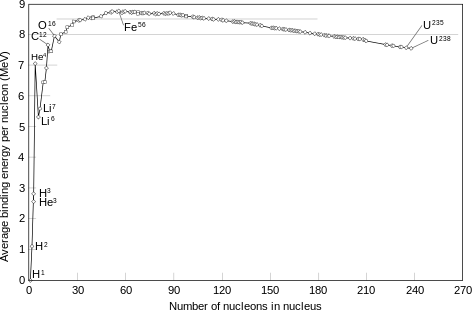
\includegraphics[width=7cm]{figures/Binding_energy.png}
\caption*{Credit: Wikipedia}
\end{figure}
\end{minipage}
}
%
\frame{
\frametitle{Coulomb barrier}

\begin{minipage}{0.4\linewidth}
\begin{itemize}
\item Nuclei have to be brought in range for the strong nuclear force
  ($10^{-15}$~m!).
\item This is opposed by the long-distance electrostatic force between
  positively charged ions.
\item To overcome this barrier the kinetic energy of the particles has
  to exceed the electrostatic potential. This happens at:
  \begin{equation}
    d = \frac{1}{4\pi \varepsilon_0} \frac{{\cal Z}_i{\cal Z}_j e^2}{\onehalf m_{\rm H} v^2}.
  \end{equation}
\end{itemize}
\end{minipage}
\hfill
\begin{minipage}{0.59\linewidth}
\begin{figure}
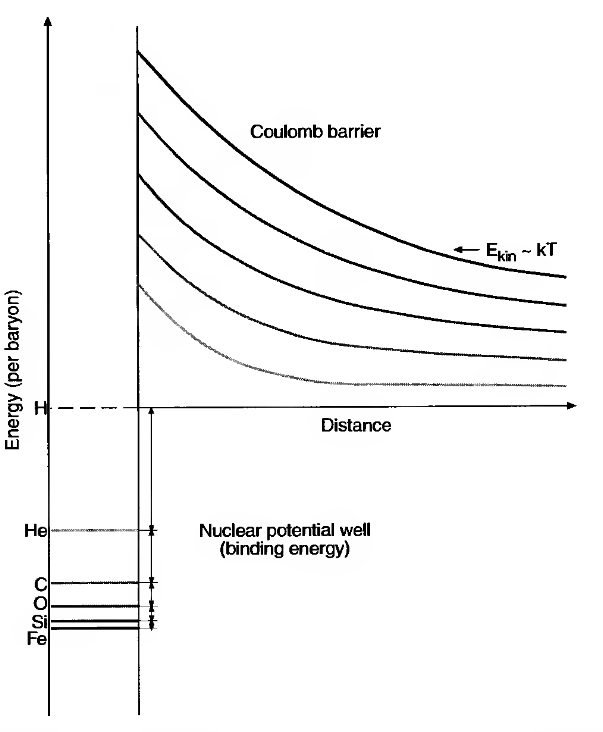
\includegraphics[width=5cm]{figures/coulomb_barrier.png}
\caption*{Credit: Prialnik}
\end{figure}
\end{minipage}
  For typical mean stellar temperatures $d$ is about $10^3$ larger
  than the range of the strong nuclear force!
}
%
\frame{
\frametitle{Gamov peak}

\begin{minipage}{0.4\linewidth}
\begin{itemize}
\item Quantum mechanical tunneling through the Coulomb barrier was
  calculated by George Gamov in 1928.
\item The tunneling probability is proportional to
  \begin{equation}
    {\rm p}_{q} \propto \exp\left\{ \frac{-\pi {\cal Z}_i {\cal Z}_j e^2}{\varepsilon_0 h v}\right\}.
  \end{equation}
\item The total probability is
  \begin{equation}
    {\rm p}_{t} \propto \exp\left\{ \frac{-\pi {\cal Z}_i {\cal Z}_j e^2}{\varepsilon_0 h v}\right\} \exp\left\{ \frac{-m_{\rm g} v^2}{2kT}\right\}.
  \end{equation} 
\end{itemize}
\end{minipage}
\hfill
\begin{minipage}{0.59\linewidth}
\begin{figure}
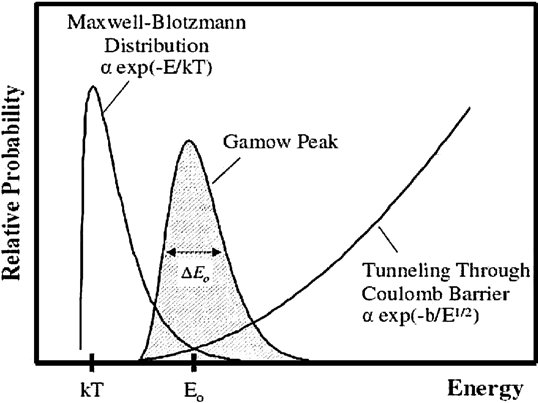
\includegraphics[width=7cm]{figures/gamow_peak.png}
\caption*{Credit: Trache (2010), Rom. J. Phys., 52, 823}
\end{figure}
\end{minipage}
This function has a maximum known as the Gamow peak which enables
fusion in stars.
}
%
\frame{
\frametitle{Hydrogen burning: $pp$ chain}
\begin{itemize}
\item Making stable helium out of hydrogen requires three or four
  protons to be brought to within $10^{-15}$~m. This is theoretically
  possible but incredibly unlikely.
\item Thus the process H $\rightarrow$ He has to go through several
  steps in a chain.
\item One such chain ($pp1$, four in total are known to exist) is
  \begin{eqnarray}
    p + p &\rightarrow& ^2{\rm D} + e^+ + \nu,\nonumber \\
    ^2{\rm D} + p &\rightarrow& ^3{\rm He} + \gamma,\nonumber \\
    ^3{\rm He} + ^3{\rm He} &\rightarrow& ^4{\rm He} + 2p.
  \end{eqnarray}
\item The $pp1$ branch works at the lowest temperatures and is
  dominant, e.g., in the Sun.
\item The energy released in the $pp$ chain is $Q_{pp} = 4\Delta {\cal
  M}(^1{\rm H}) - \Delta {\cal M}(^4{\rm He}) = 26.73$~MeV.
\item Rate of energy release is roughly proportional to
  \begin{equation}
    q_{pp} \propto \rho T^4.
  \end{equation}
\end{itemize}
}
%
\frame{
\frametitle{Hydrogen burning: CNO cycle}
\begin{itemize}
\item Another process that can fuse hydrogen to helium is the CNO
  (carbon-nitrogen-oxygen) cycle (Bethe, von Weizs\"acker, 1938). 
\item Here the CNO elements act as catalysts that enable the fusion H
  $\rightarrow$ He, and they are neither destroyed or created in the
  process:
\begin{figure}
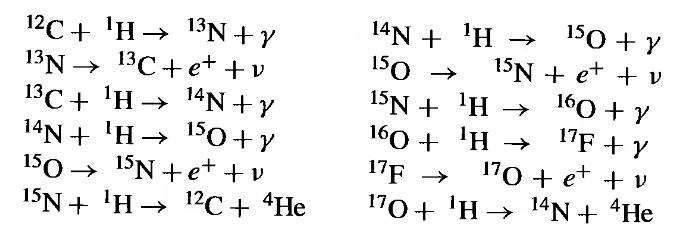
\includegraphics[width=8cm]{figures/CNO-cycle.png}
\caption*{Credits: Prialnik}
\end{figure}
\item $Q_{\rm CNO} \approx 25$~MeV, and rate of energy release is
  (very) roughly:
  \begin{equation}
    q_{\rm CNO} \propto \rho T^{16}.
  \end{equation}
\item Steep $T$ dependence will have repercussions for stellar
  structure (next lecture).
\end{itemize}
}
%
%
\frame{
\frametitle{Helium burning: Triple $\alpha$ reaction}
\begin{itemize}
\item The triple $\alpha$ reaction proceeds in two steps:
  \begin{eqnarray}
    ^4{\rm He} + ^4{\rm He} &\rightarrow& ^8{\rm Be},\nonumber \\
    ^8{\rm Be} + ^4{\rm He} &\rightarrow& ^{12}{\rm C}.
  \end{eqnarray}
\item This reaction occurs despite $^8$Be having a lifetime of only
  $2.6\cdot10^{-16}$~s!
\item Rate of energy release is extremely sensitive to $T$:
  \begin{equation}
    q_{\rm CNO} \propto \rho^2 T^{40}.
  \end{equation}
\item However, also the ignition temperature is high ($\approx
  10^8$~K).
\end{itemize}
}
%
%
\frame{
\frametitle{Summary of the most common fusion processes}
\begin{minipage}{0.4\linewidth}
\begin{itemize}
\item $pp$ chain dominates in low mass stars such as the Sun.
\item CNO cycle is operating in more massive main-sequence stars.
\item The first stars generated also heavier elements from triple
  $\alpha$ (and subsequent) reactions.
\end{itemize}
\end{minipage}
\hfill
\begin{minipage}{0.59\linewidth}
\begin{figure}
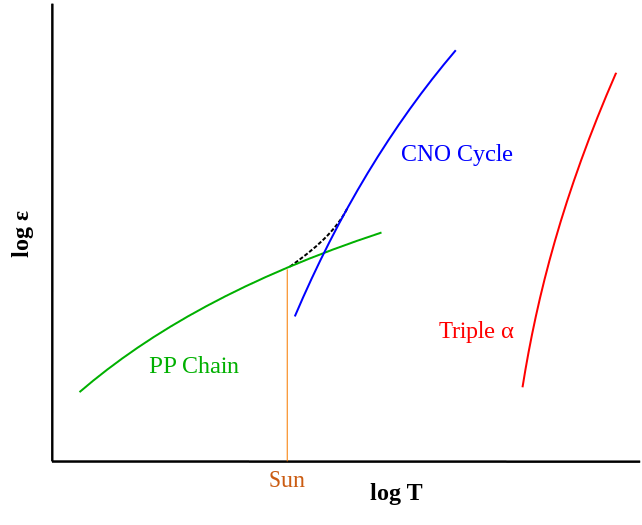
\includegraphics[width=7cm]{figures/Nuclear_energy_generation.png}
%\caption*{Credit: RJHall, https://en.wikipedia.org/wiki/File:Nuclear\_energy\_generation.svg}
\end{figure}
\end{minipage}
Credit: RJHall, https://en.wikipedia.org/wiki/File:Nuclear\_energy\_generation.svg (CC-SA 3.0)
}
%
%% %
%% \frame{
%% \frametitle{Solar spectrum is NOT a blackbody spectrum}
%% \begin{figure}
%% 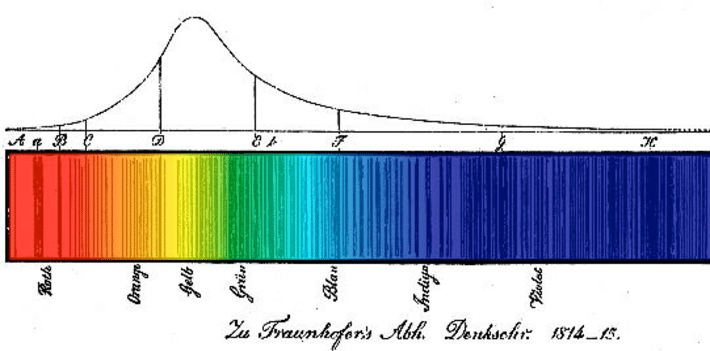
\includegraphics[width=6cm]{figures/fraunhofer_spectrum.png}
%% \caption*{Credits: Fraunhofer (1814)}
%% \end{figure}
%% \begin{itemize}
%% \item These lines represent loss of light at specific wavelengths - solar atmosphere is much more opaque at these wavelengths. \q{Why?}
%% \item Kirchoff and Bunsen (1860's) related them to chemical elements. 
%% \item Birth of quantum mechanics: Bohr's model can explain hydrogen lines. \textbf{Energy jumps between discrete energy levels}.
%% \item Discovery of Helium by Janssen (1868) in the solar spectrum.
%% \end{itemize}
%% }
%
%
\end{document}



